\chapter{Camera and \acs{lidar} Calibration}
\label{chapter:calibration}

This chapter focus is on sensory calibration. The experimental setup is described, the method used to calibrate the camera and \ac{lidar} intrisic parameters are detailed. Finally, after proper calibrated, the two sensors can be calibrated amongst themselves, on a extrinsic calibration procedure. This procedure is explained from a mathematical standpoint and the implementation is shown, along some results.


\section{Experimental Setup}
The experimental setup is shown on figure~\ref{fig:experimental-setup}. It consists of an industrial camera and C-mount lens, \ac{tof} \ac{lidar}, router and power source (not shown on the figure). 

The camera model used is an industrial 5\ac{mp} RGB camera, from Allied Vision, Manta G504C. Camera lens is a 1'' C-Mount Format Camera with Lock from Thorlabs\cp, MVL16M1. The full camera specifications can accessed on~\cite{MantaG504C} and the full lens specifications on~\cite{Thorlabs}. Relevant specifications of the camera and lens can be found on table~\ref{tab:camera-and-lens-specs}. 

\begin{table}[H]
	\renewcommand{\arraystretch}{1.2}
	\centering
	\begin{tabular}{@{}lp{7cm}l@{}}
		\toprule
		\multicolumn{2}{l}{Specification} & Value \\ \midrule
		\multicolumn{2}{l}{\emph{Camera}} & \\
		\phantom{a} & Full Resolution (width vs heigth) & $2452 \times 2056$   \\
									& Shutter mode & Global \\
									&	Maximum \ac{fps} at full resolution & $9.2$ \\ \midrule 
									\multicolumn{2}{l}{\emph{Lens}} \\
									&	Focal Length & $16$ mm \\
									&	Max aperture & $f/1.4$ \\
									&	Minimum Object Distance & $300$ mm  \\
									& \acs{adc}\footnotemark bit depth & $12$ bit \\
		\bottomrule
	\end{tabular}
	\caption{Relevant specifications for AVT Manta G504C RGB camera (from~\cite{MantaG504C})  and MVL16M1 Thorlabs\cp lens (from~\cite{Thorlabs}).}
	\label{tab:camera-and-lens-specs}
\end{table}

\footnotetext{\acs{adc} stands for \acl{adc}}

The \ac{tof} \ac{lidar} used is a Velodyne VLP-16\texttrademark. VLP-16 is a 16 beam \ac{lidar} that operates at 903nm, supporting various return modes (Strongest, Last, Dual) and allowing its connection with a \ac{gps} for positioning and synchronization. It aslo supports several rotation velocities. The full specifications can be seen on~\cite{VLP16} and the relevant specifications for this work are summarized on table~\ref{tab:vlp16-specs}.

\begin{table}[H]
	\renewcommand{\arraystretch}{1.2}
	\centering
	\begin{tabular}{@{}p{6cm}l@{}}
		\toprule
		Specification & Value \\ \midrule
		Wavelength    & 903nm \\
		Motor \acs{rpm}\footnotemark & $600 \pm 3$ \\
		Angular step & 0.2º \\
		Maximum Scanning Distance & 100m \\
		Max Error & $2 cm$ \\
		\bottomrule
	\end{tabular}
	\caption{Velodyne VLP-16 relevant specifications. Source~\cite{VLP16}.}
	\label{tab:vlp16-specs}
\end{table}

\footnotetext{\acs{rpm} stands for \acl{rpm}}

Both VLP-16 and Manta G-504C operate over Gibabit Ethernet. Therefore, a Gibabit switch is required to connect all the equipment to a single computer using a single Ethernet port. The switch used was Cisco SG200-08, a 8-Port Gigabit Smart Switch. It was configured so that every port was on the same \ac{vlan}, ensuring packets were accessibel on the computer. An alternative was to redirect the packets from each sensor to the computer network and filter which packets reached each sensor. Since no bandwidth constraints, packet delay/loss or higher ping time problems arised, the solution chosen was the former, due to its simplicity. For each device a fixed \ac{ip} address as attributed, following the intructions on their datasheet~\cite{VLP16, MantaVision2013} and the \acp{ip} addresses can be consulted on table~\ref{experimental-setup-ip}.

\begin{table}[H]
	\renewcommand{\arraystretch}{1.2}
	\centering
	\begin{tabular}{@{}lcc@{}}
		\toprule
		Device          & \ac{ip} Adress & Subnet Mask\\ \midrule
		Computer        & 192.168.10.77  & 255.255.255.0 \\
		Manta G-504C    & 192.168.10.1   & 255.255.255.0 \\
		Velodyne VLP-16 & 192.168.10.201 & 255.255.255.0 \\
		\bottomrule
	\end{tabular}
	\label{tab:experimental-setup-ip}
	\caption{\acp{ip} and subnet masks for the devices connected on the experimental setup.}
\end{table}

To power the Manta G-504, a laboratory power source must be used. Manta consumes $3.9 W$~\cite{MantaG504C} while operating and access a input voltage between $8$ and $30$ $V_{DC}$. The power source used was set to  $12 V_{DC}$ and the current output was $\approx 0.3$. Voltage and current were measured during all tests, and summaried results are presented on table~\ref{tab:matna-power}. Manta power cable used is a U20 \ac{udp} cable with a HIROSE HR10A-10P-12S female connector. Since the mapping from the 8 pins \ac{udp} cable to the 12 pin connector was not available, a continuity test was made between the expected pinout of the power cable (for more details, see~\cite{AVTCables}) and the real pinout. The results can be consulted in~\nameref{sec:appendix-b}, on table~\ref{tab:manta-power-cable-pinout}.

	
\begin{table}[H]
	\centering
	\renewcommand{\arraystretch}{1.2}
	\renewcommand{\tabcolsep}{0.45cm}
	\begin{tabular}{@{}llll@{}}
		\toprule
					  & Minimum & Maximum & Median Value \\ \midrule
		Current ($mA$) & $298 \pm 1$ & $330\pm 1$ & $312 \pm 1$ \\
		Voltage ($V$)  & $12.00\pm 0.07 $ & $12.18\pm 0.07$ & $12.08\pm0.07$ \\
		\bottomrule
	\end{tabular}
	\centering
	\label{tab:manta-power}
	\caption{Voltage and Current measurements during Manta AVT G-504C operation. Minimum and Maximum values were registered, along with the median. }
\end{table}

The physical setup was constructed using Thorlabs\cp Optomechanic material to mount the camera and \ac{lidar}. The final setup can be seen on figure~\ref{fig:experimental-setup}.

\begin{figure}[H]
	\centering
	\begin{subfigure}[c]{0.45\textwidth}
		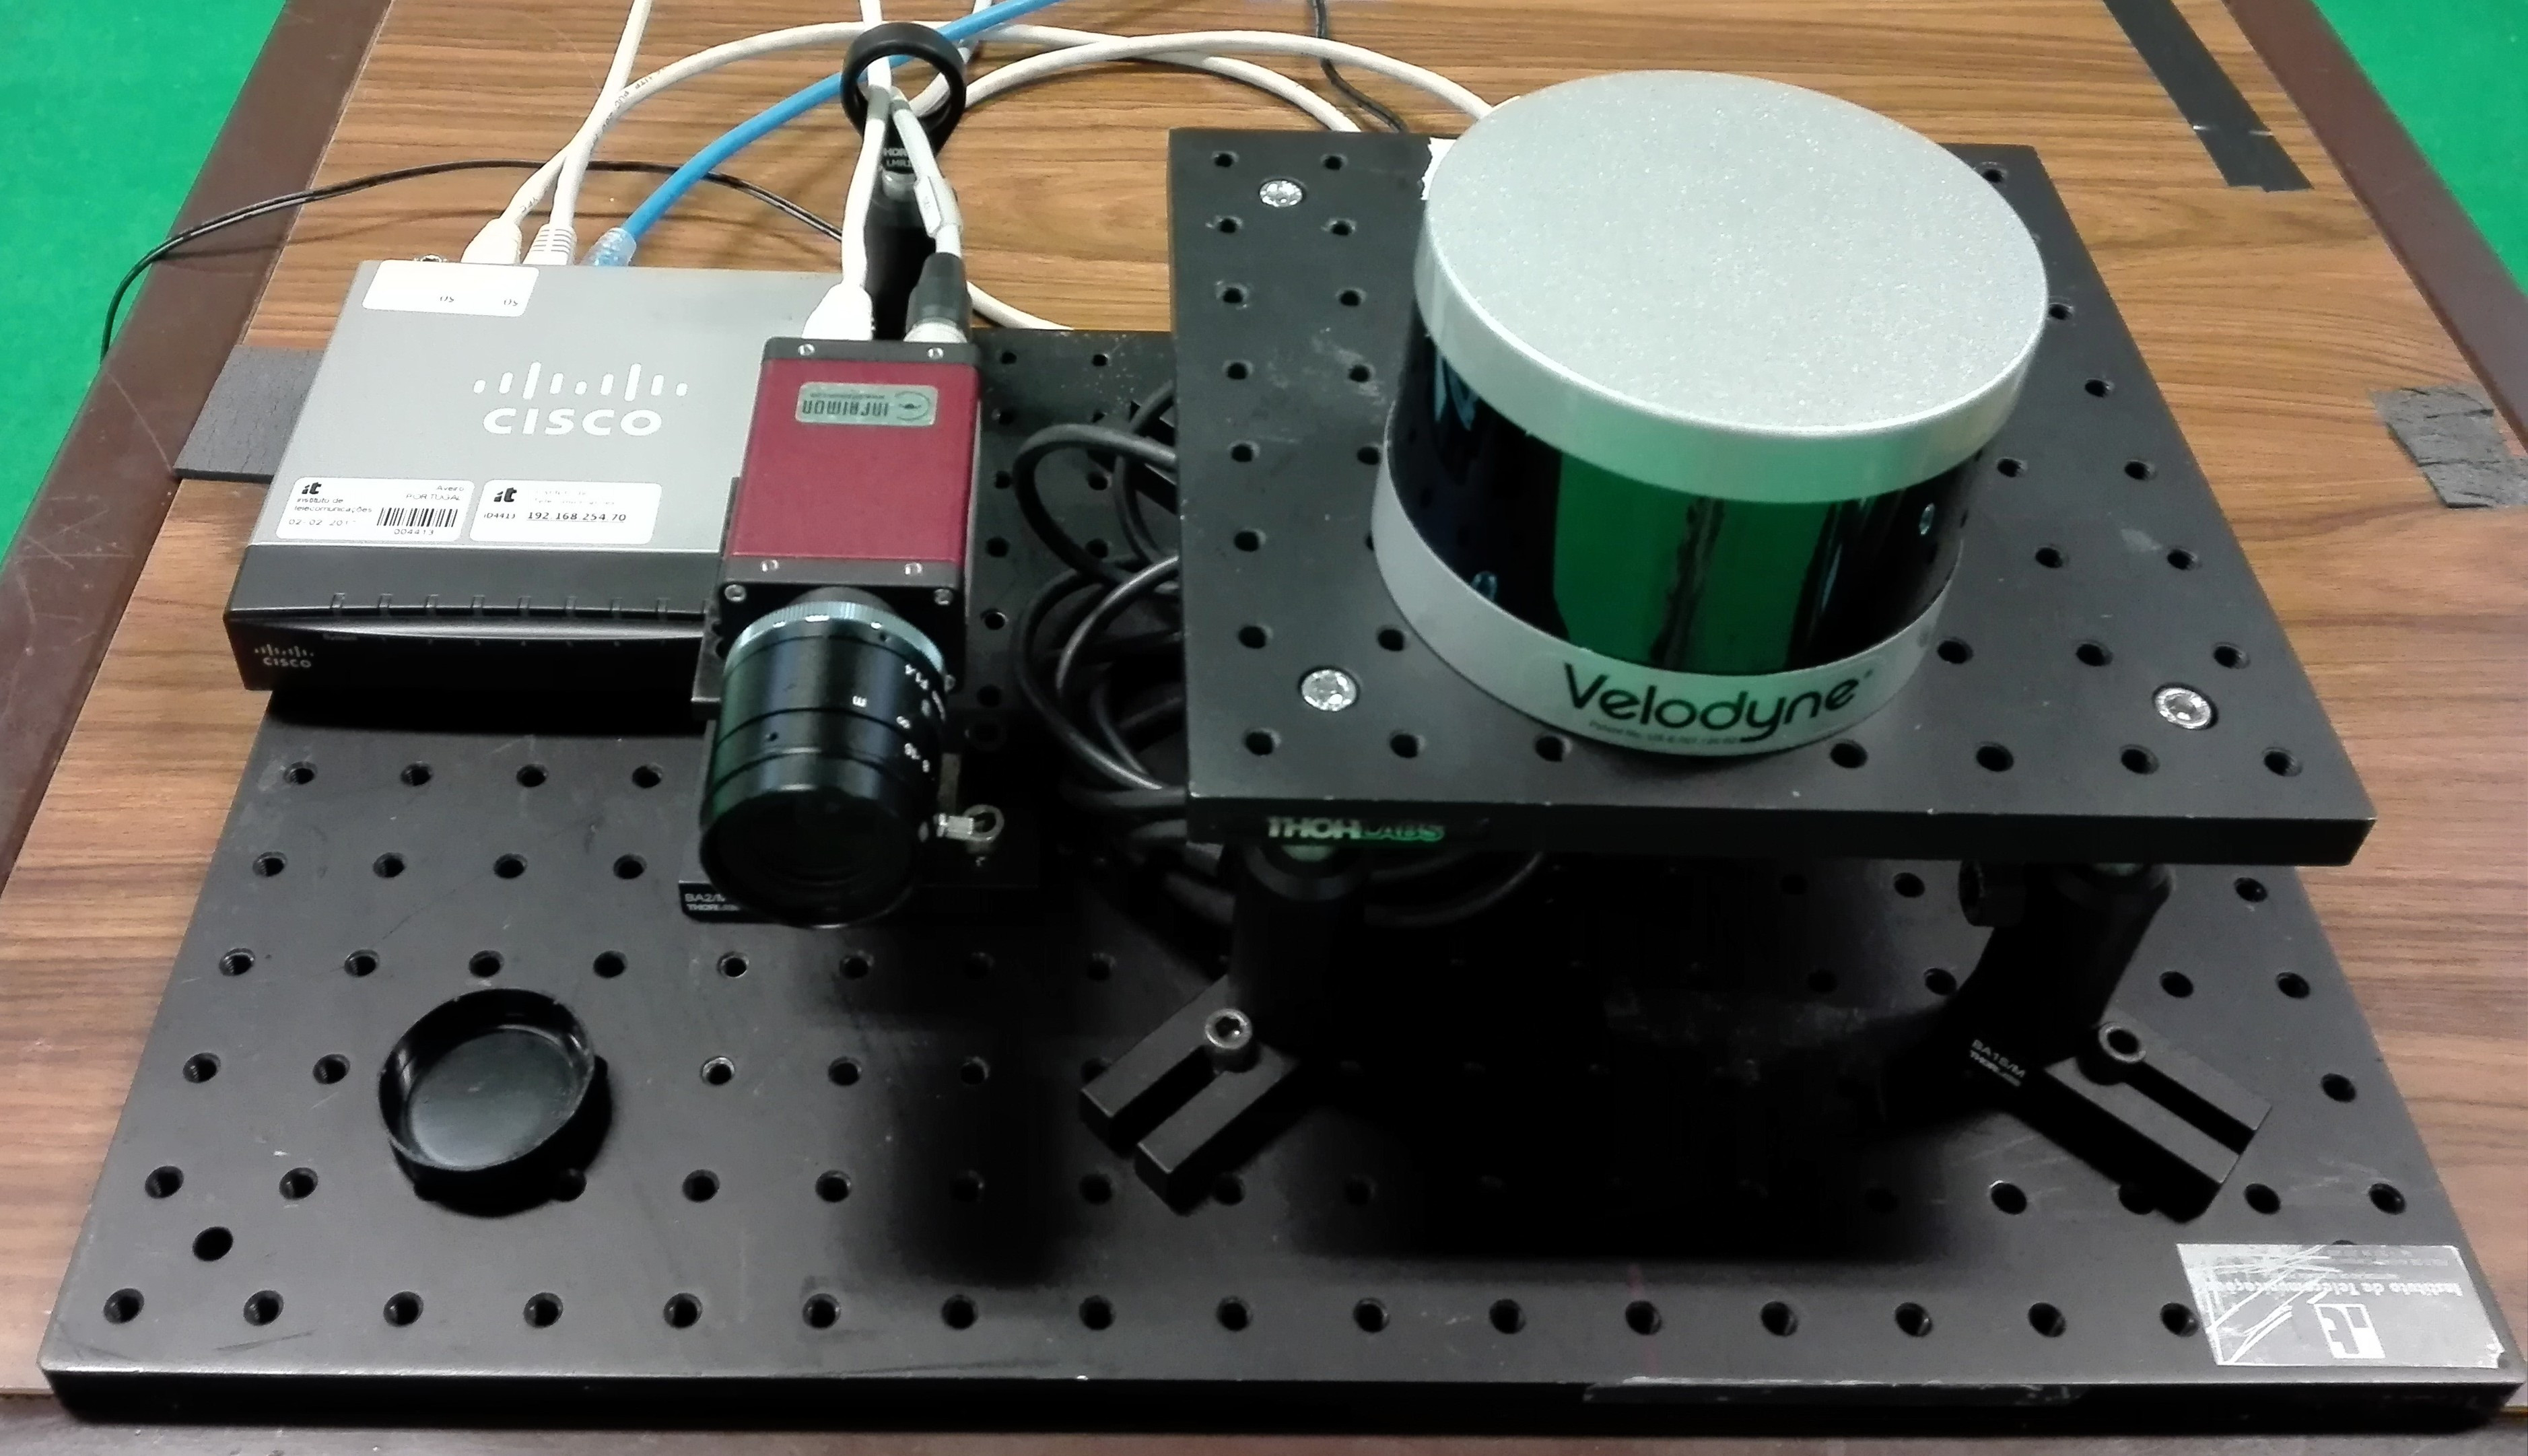
\includegraphics[width=\textwidth]{img/experimental-setup/table-setup-cambada-perspective.jpg}
		\caption{Experimental Setup viewed in perspective.}
		\label{fig:experimental-setup:perspective}
	\end{subfigure}
	\qquad
	\begin{subfigure}[c]{0.45\textwidth}
		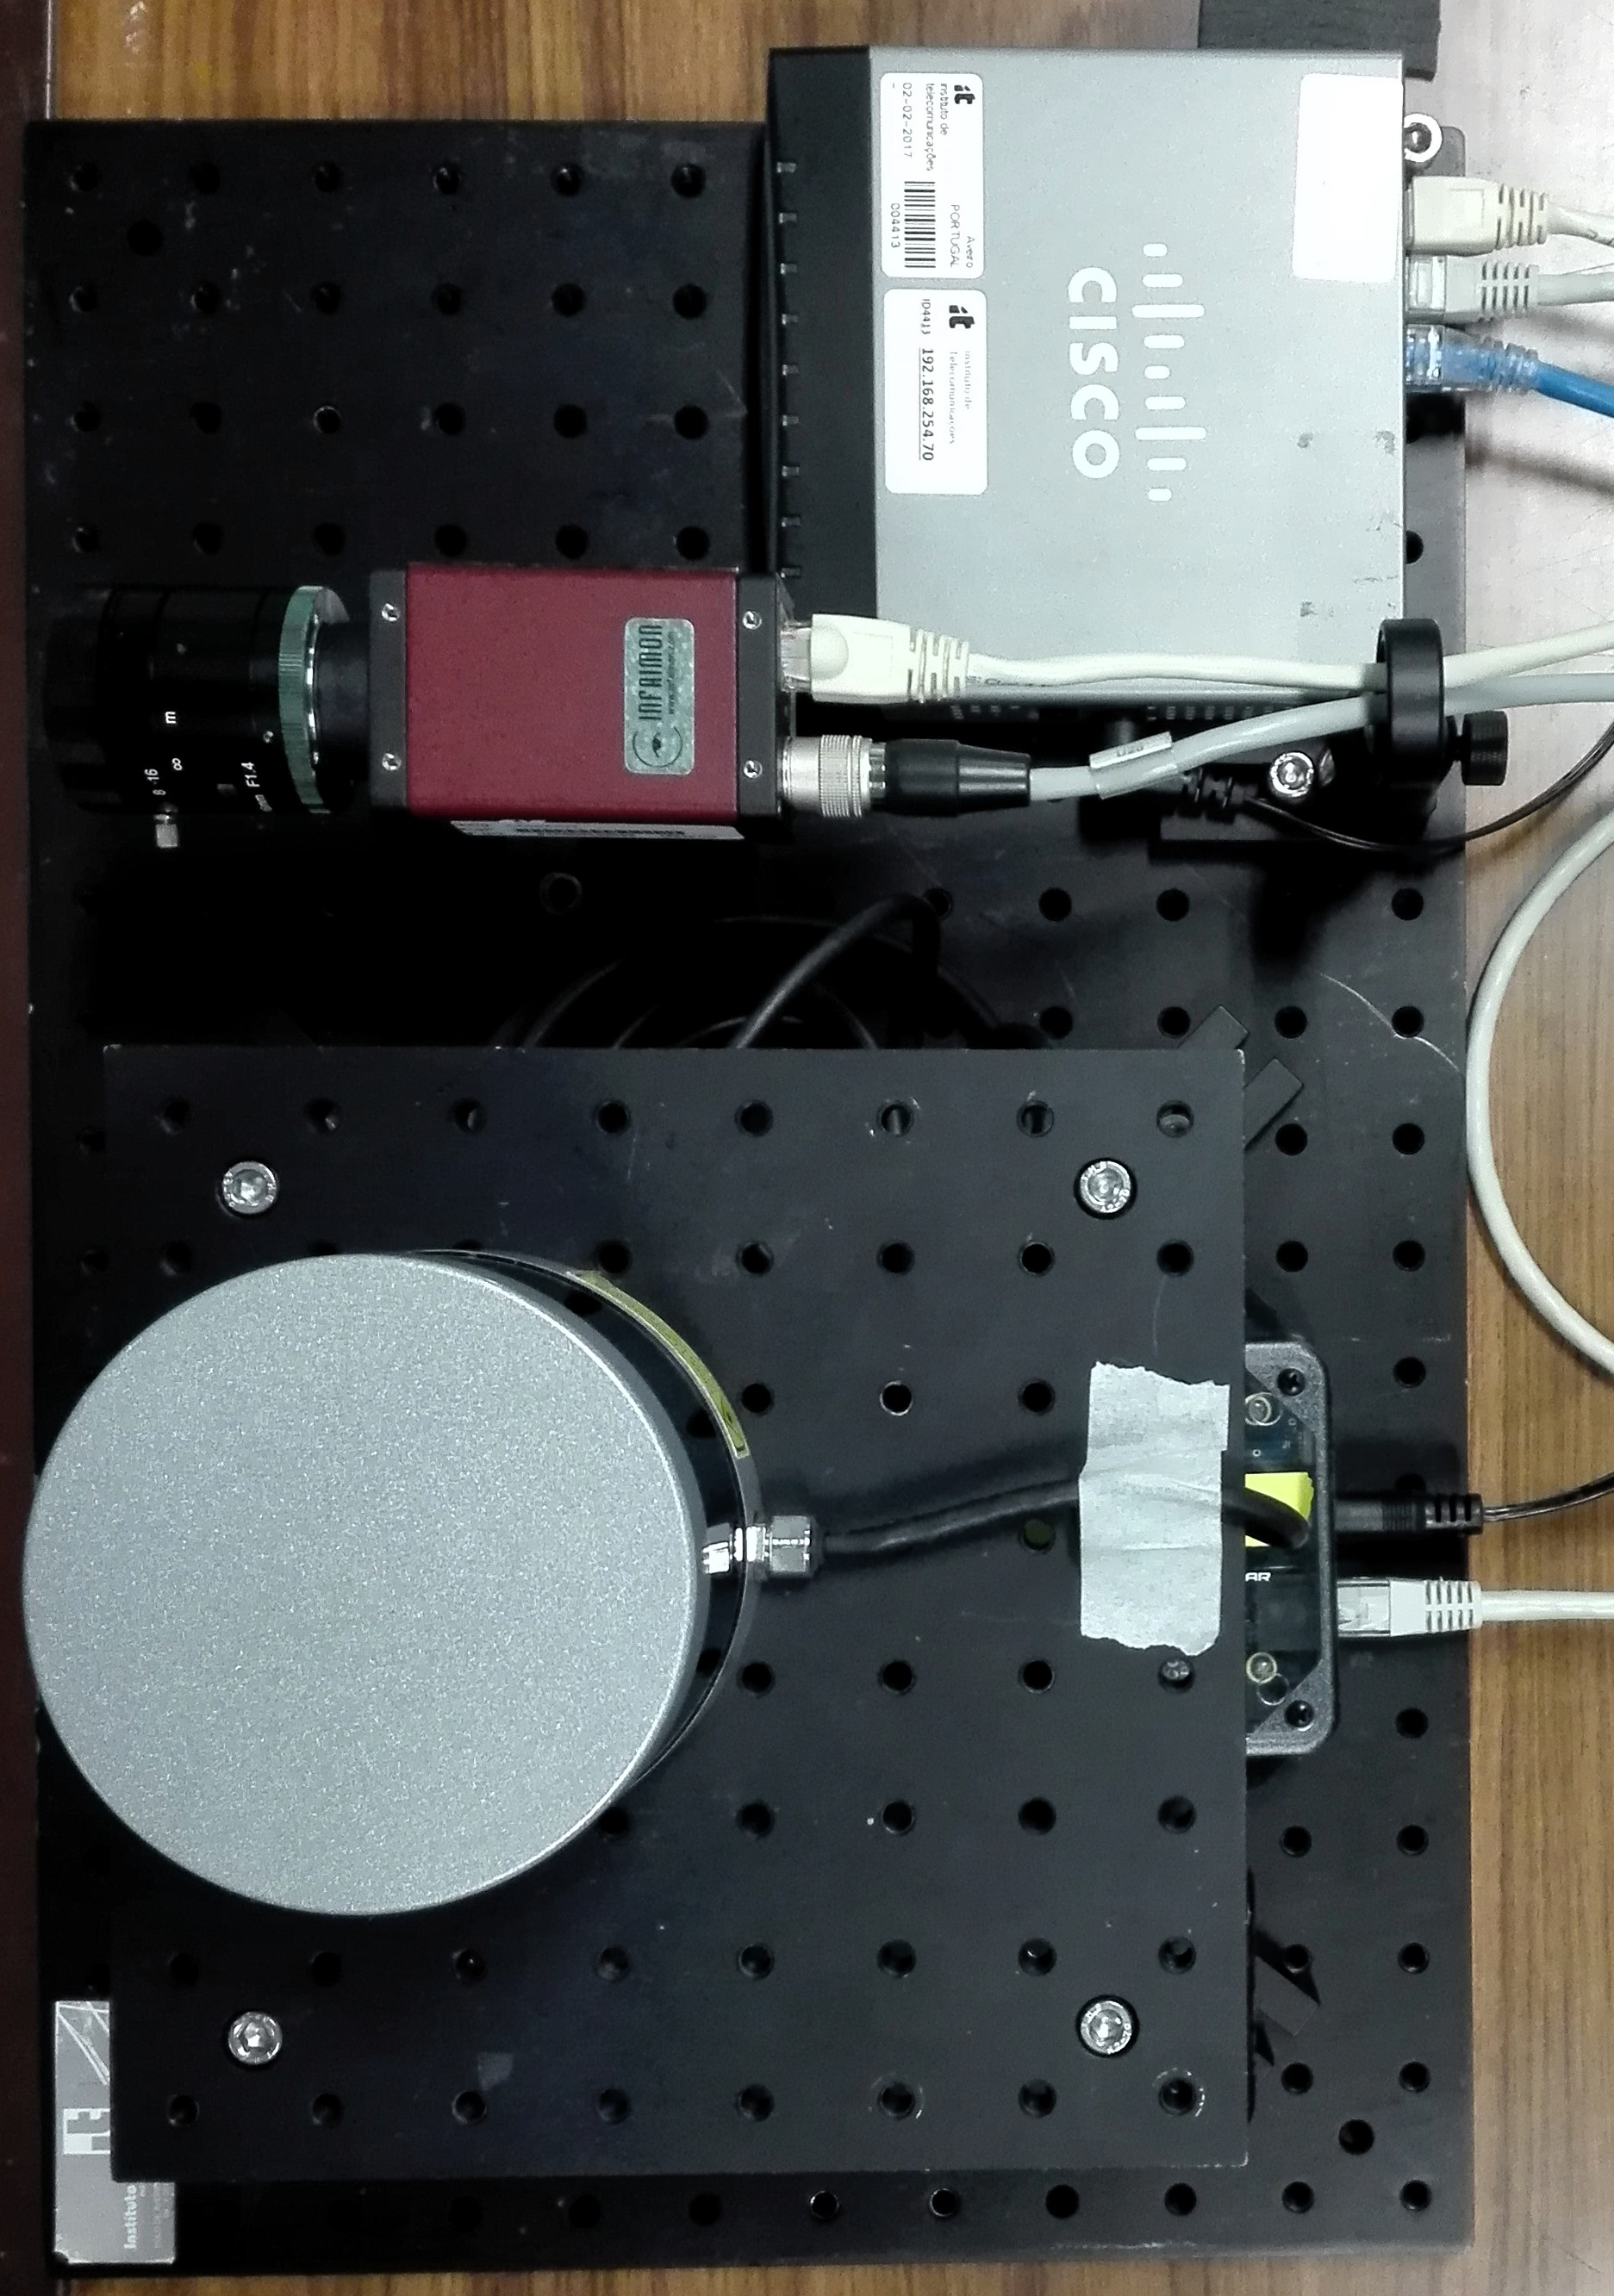
\includegraphics[width=0.65\textwidth, keepaspectratio, angle=90]{img/experimental-setup/table-setup-cambada-birds-eye.jpg}
		\caption{Experiemental Setup from a bird's eye view.}
		\label{fig:experimental-setup:birds-eye}
	\end{subfigure}
	\caption{Experimental Setup from a bird's eye view.}
	\label{fig:experimental-setup}
\end{figure}

No significant interference is expected between the camera and \ac{lidar}. The camera lens was a tranmission shown at figure~\ref{fig:lens-transmission}, that at $900 nm$ is $66\%$. However, Sony ICX655, the Camera Sensor of Manta G-504C, only was a Quantum Efficiency of $\approx 6\%$~\cite{MantaG504C}.

\begin{figure}[H]
	\centering
	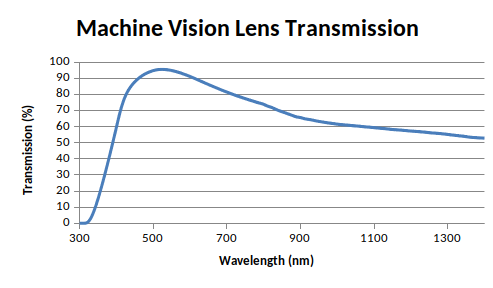
\includegraphics[width=0.6\textwidth]{img/experimental-setup/lens-transmission.png}
	\caption{Transmission of the MVL16M1 lens in relation the light wavelength. Source~\cite{Thorlabs}}
	\label{fig:lens-transmission}
\end{figure}



\section{Camera Intrinsic Calibration}
As stated on Section~\ref{subsec:sota:camera-intrinisc-calibration}, the act of calibrating a camera consists on determining its intrinsic parameters. This can be done by taking different images with a know pattern fully visible on the camera \ac{fov}, changing its rotation an translation relating tho the camera.

The calibration procedure uses a chessboard of $13 \times 9$ squares, with each square having a edge length of $44.0mm$. The chessboard used can be seen on figure~\ref{fig:chessboard}. It was laser printed and then glued to a plywood board.

\begin{figure}[H]
	\centering
	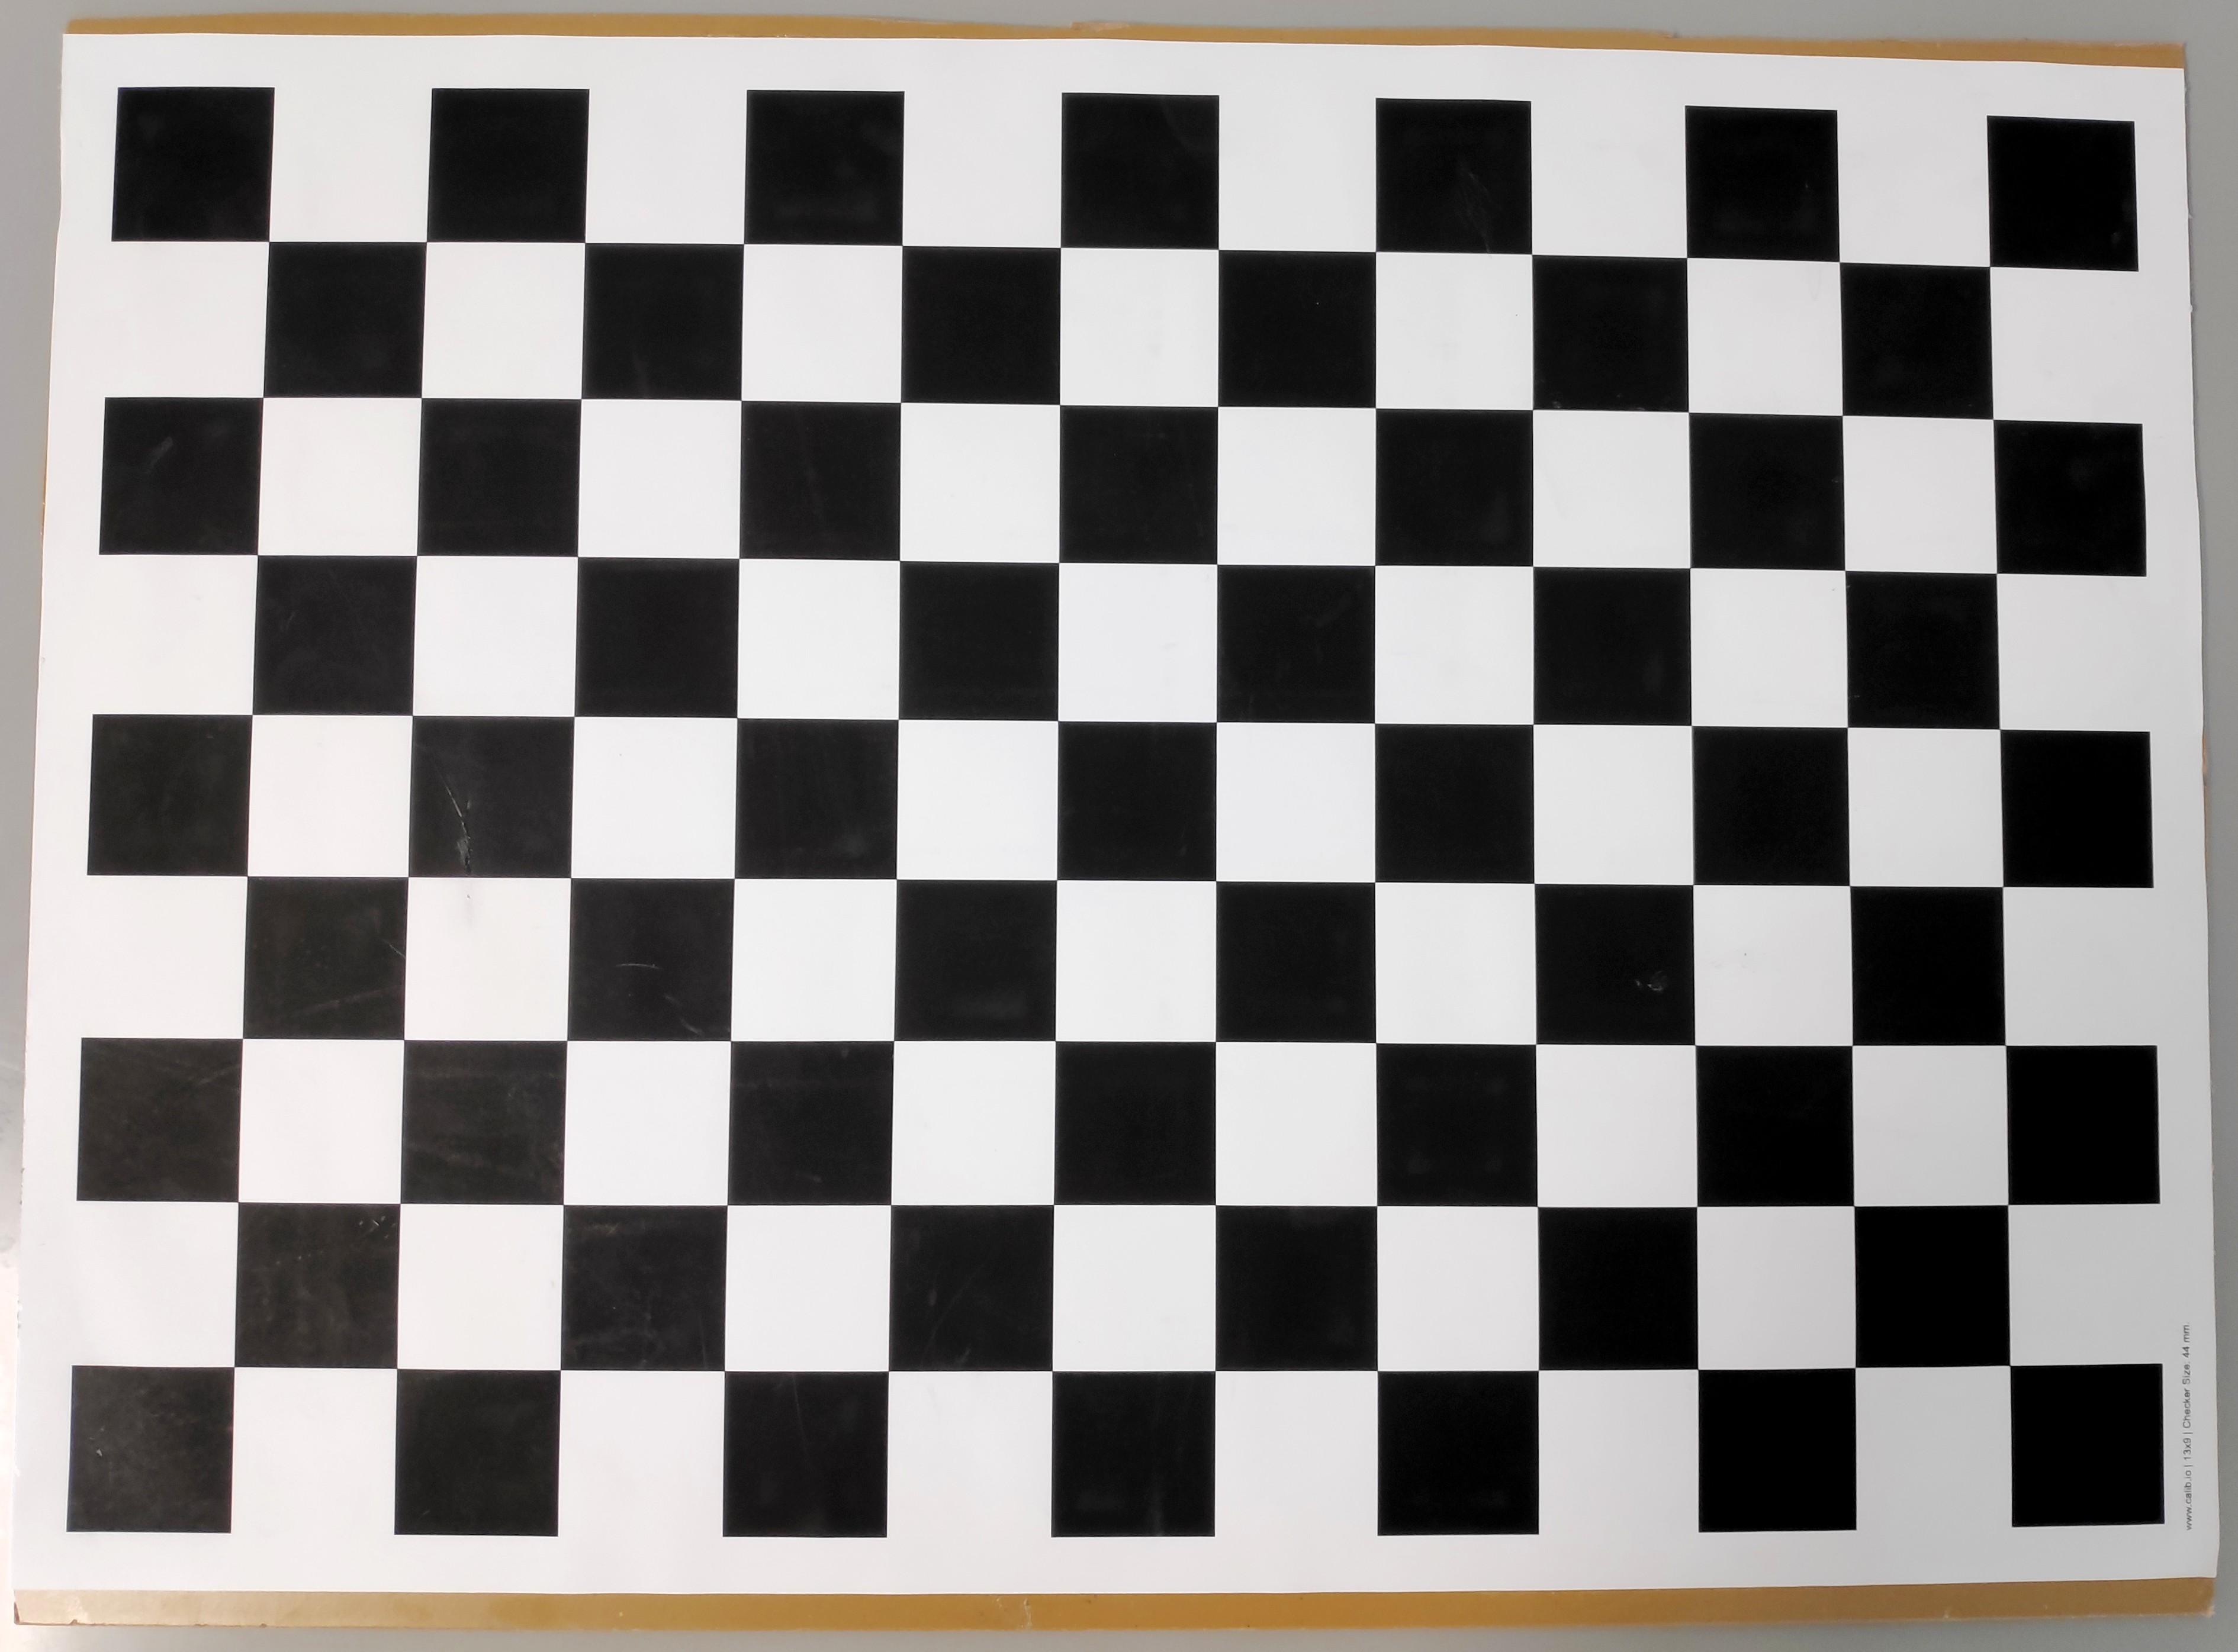
\includegraphics[width=0.5\textwidth]{img/experimental-setup/chessboard.jpg}
	\caption{Chessboard used during camera calibration procedures. The chessboard was laser printed on a A1 paper, in real size, that was glued to a plywood board.}
	\label{fig:chessboard}
\end{figure}

However, before any propoer calibration can me made, the camera must be focused. The focus theory and procedure are layed out on the next sub-section,~\ref{subsec:calibration:camera-focus}.


% Therefore, to proper use a camera on the field of computer vision, some notions of photography are required. Since this research is focused on the usage of industrial cameras and not consumer cameras, such notions will be simplified to the minimum necessary. 

\subsection{Camera Focus and \acl{dof}}
\label{subsec:calibration:camera-focus}
Focusing a camera can only be attained for an exact distance from the camera~\cite{Merklinger1993, Photopillers}, measured perpendicularly to the plane of focus, which is the plane containing the \ac{cmos} or \ac{ccd} chip. Therefore, on every image, there is a plane of focus and what actually ``looks focused'' is really just ``acceptably sharp focus'', since precise focus is only possible to an exact distance, and not for an entire tridimensional object.

``Acceptably sharp focus'' means that a point in the real world would not result in a point on the image (as happens in precise focus), but in a blurred spot that is circular (due to the form of the aperture)\cite{Photopillers}. However, if the size of blur is small enough, little to no differences can be perceived and the image is considered to be focused\cite{Photopillers}. The maximum size at which this blur is not noticed by the viewer (given a specific sensor size, dimension of the viewed photo, viewing distance and acuity of the viewer) is called the \ac{coc}\cite{Photopillers, Merklinger1993}.

The first step in focusing an image requires the calculation of the hyperfocal distance, $H$: the distance at which the camera is focused to ensure objects from half of this distance to the infinity are in an ``acceptably sharp focus'' (refer to as just focus, from now on). This distance can be calculated using the equation~\ref{eq:hyperfocal_distance}, below, where $f$ is the focal length, $N$ is the F-number and $c$ the \ac{coc} limit. Hyperfocal near limit is defined as $H_{near} = \frac{H}{2}$.

\begin{equation}
	\label{eq:hyperfocal_distance}
	H = \frac{f^2}{Nc} + f \approx \frac{f^2}{Nc} 
\end{equation}

Known the hyperfocal distance, the \acf{dof} can be calculated. \ac{dof} is measured in meters and is the subtraction of the farthest and nearest distance at each object is focused (see equation~\ref{eq:dof}), indicating the distance between this two points\cite{Photopillers, Merklinger1993, mvg_book}. The nearest and farthest points can be calculated using the equations~\ref{eq:dof_near} and~\ref{eq:dof_far}, respectively.

\begin{subequations}
	\label{eq:dof_all}
	\begin{align}
		DoF & = DoF_{far} - DoF_{near} \label{eq:dof} \\
		DoF_{far} & = \frac{H\times d}{H - (d - f)} \label{eq:dof_far} \\
		DoF_{near} & = \frac{H\times d}{H + (d - f))} \label{eq:dof_near} 
	\end{align}
\end{subequations}

Using equations~\ref{eq:dof_all} is possible to select a desired \acl{dof} for an image that guarantees that all the objects of interest are focused. Taking in consideration that smaller apertures (bigger F-numbers) will increase the exposition time\cite{Merklinger1993}, a target distance can be selected with the guarantee that all the objects from the near \ac{dof} point to the far \ac{dof} will be sharp.

\subsection{Camera Calibration Procedure}

\subsection{Camera Calibration Results}

\section{\ac{lidar} Intrinsic Calibration}
Apply table of calibration 

Calibrated against NI qq coisa
